\documentclass[border=2pt]{standalone}
\usepackage{amsmath, amsthm, amsfonts}
\usepackage{tikz-cd, kotex}
\usepackage{quiver}
\usepackage{Operators}
\usepackage{palette}
\usepackage{diagram-style}
\begin{document}

%%FIG decomposition (Schemes-1.svg)
\begin{tikzcd}
	\Spec A_f\rar["\Spec\epsilon"]\drar[sloped, swap, "\sim" above]\drar["\Spec\epsilon\vert^{D(f)}" {below, xshift=-12pt, yshift=-3pt}]&\Spec A\\
	&D(f)\uar[hook, "\iota" right]
\end{tikzcd}

%%FIG line_with_two_origins (Schemes-2.svg)
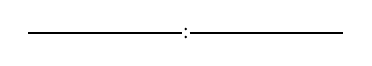
\begin{tikzpicture}
	\draw (-2,0)--(-.05,0);
	\draw (.05,0)--(2,0);
	\fill (0,0.05) circle[radius=.5pt];
	\fill (0,-.05) circle[radius=.5pt];
\end{tikzpicture}

%%FIG projective_line (Schemes-3.png)
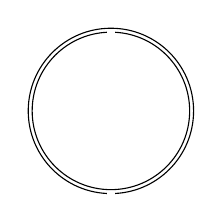
\begin{tikzpicture}
	\draw (0,0) circle[radius=1];
	\draw (0,0) circle[radius=1.05];
	\draw[white, very thick] (-.05,1)--(.05,1);
	\draw[white, very thick] (-.05,-1.05)--(.05,-1.05);
\end{tikzpicture}

\end{document}
